\documentclass[10pt,a4paper,openany,twoside]{book}

\usepackage{layout_cours}
\usepackage{hyperref}
\setlist{leftmargin=5mm}

\begin{document}
	\chapnumber{3} % numéro du chapitre
	\titre{Suites géométriques} % titre du chapitre
	\classe{Terminale STMG} % classe
	\entetegal


\section{Formule de récurrence}

\begin{defi}{Suite géométrique}{}
	Une suite est dite \textbf{géométrique} lorsqu'on passe d'un terme au suivant en multipliant à chaque fois par un même nombre $q\in\R$ appelé \textbf{raison} de la suite.

	\noindent Une suite géométrique est définie par la donnée de son premier terme (généralement $u_0$ ou $u_1$) et la relation de récurrence :
	\[ \left\lbrace
	\begin{array}{l}
		u_0\in \R\\
		u_{n+1} = u_n \times q\\
	\end{array}
	\right. \]
	\begin{center}
		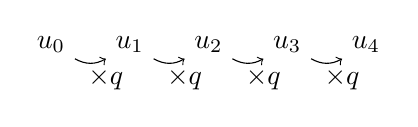
\begin{tikzpicture}
			\node[above] (A) at (0,0) {$u_0$};
			\node[above] (B) at (1,0) {$u_1$};
			\node[above] (C) at (2,0) {$u_2$};
			\node[above] (D) at (3,0) {$u_3$};
			\node[above] (E) at (4,0) {$u_4$};
			\draw[->] (A) to [bend right] (B) node[below]  {$\times q$};
			\draw[->] (B) to [bend right] (C) node[below]  {$\times q$};
			\draw[->] (C) to [bend right] (D) node[below]  {$\times q$};
			\draw[->] (D) to [bend right] (E) node[below]  {$\times q$};
		\end{tikzpicture}
	\end{center}
\end{defi}

\begin{ex}{Echiquier de Sissa}{echiquier}
 On place un grain de riz sur la première case d'un échiquier. On fait en sorte de doubler à chaque case le nombre de grains de la case précédente. Alors si on appelle $(v_n)$ la suite qui donne le nombre de grains sur chaque case, cette suite est géométrique de raison $q=2$ et de premier terme $v_1=1$.
\end{ex}

\begin{ex}{Intérêts composés}{interets_composes}
	Au 1er janvier 2026, on place un capital de 1500€ à intérêts composés sur un livret au taux de 2\% par an. On note $u_n$ le capital sur le compte au 1er janvier (2026+n).

	Le premier terme de la suite $(u_n)$ est $u_0 = 1500$.
On passe d'un terme au suivant en multipliant par $1.02$. On obtient $u_{n+1} = u_n \times 1.02$.

$(u_n)$ est donc une suite géométrique de raison $q=1.02$ et de premier terme $u_0=1500$.
\end{ex}

\begin{methode}{Prouver que trois nombres $u_0$, $u_1$ et $u_2$ suivent une progression géométrique}{}
\begin{enumerate}
	\item On calcule le quotient entre les termes consécutifs, c'est-à-dire $u_1/u_0$ et $u_2/u_1$
	\item
	Si cette différence est constante, c'est-à-dire $u_1/u_0 = u_2/u_1$, alors les trois termes $u_0$, $u_1$ et $u_2$ suivent une progression géométrique.
\end{enumerate}
\end{methode}

\begin{ex}{}{}
Soient les termes $v_1=7$, $v_2=-14$, $v_3=28$.

On calcule $v_2/v_1=28-14/7=-2$ et $v_3/v_2=28/(-14) =-2$. On conclut qu'ils ne suivent pas une progression géométrique.
\end{ex}

\begin{defi}{Moyenne géométrique}{}
	La \bf{moyenne géométrique} $m$ de deux nombres $a\in\R$ et $b\in\R$ est donnée par :
	$$m = \sqrt{ab}$$
\end{defi}

\begin{ex}{}{}
  La moyenne géométrique de $a=12$ et $b=3$ est $m=\sqrt{12\times 3 }=\sqrt{36}=6$
\end{ex}

\begin{ex}{}{}
	Soit $(w_n)$ une suite géométrique de raison 1.5 et de premier terme $w_1=7$.
	
	On calcule $w_2=10.5$ et $w_3=15.75$. La moyenne géométrique de $w_1$ et $w_3$ est alors $m=\sqrt{w_1 \times w_3} = \sqrt{7\times15.75}=10.5$. On observe qu'on a $m = w_2$.
\end{ex}

\begin{rem}{}{}
  Plus généralement, chaque terme d'une suite géométrique est la moyenne géométrique des termes qui l'encadrent.
\end{rem}

\begin{ex}{}{}
		On peut comparer cette moyenne avec la moyenne arithmétique, $M = \frac{w_1+w_3}{2} = \frac{7+15.75}{2} = 11.37$. En général, les deux moyennes ne sont pas égales.
\end{ex}

\section{Terme général}

\begin{theo}{Terme général d'une suite géométrique}{}
Soit$(u_n)$ une suite géométrique de raison $q$ et de premier terme $u_0$.

On a pour tout $n\in\N$, $$u_n=u_0\times q^n$$

Si le premier terme est $u_1$, on a $u_n=u_1\times q^{n-1}$
\end{theo}

\begin{dem}{}{}
Si $(u_n)$ est géométrique de raison $q$, pour passer de $u_0$ à $u_n$, on multiplie $n$ fois par la raison $q$ donc $u_n=u_0\times \underset{n \text{ fois}}{\underbrace{q \times q \times \cdots \times q }}= u_0\times q^n$.
\end{dem}

\begin{rem}{}{}
  On peut vérifier sa formule en calculant le premier terme:

  Pour $n=0$, on obtient $u_n=u_0\times q^0 =u_0 \times 1 = u_0$.
\end{rem}

\begin{ex}{}{}
	En reprenant l'exemple \ref{exe:interets_composes}, on calcule $u_n = u_0\times q^n = 1500\times {1.02}^n$.

	On peut alors calculer l'argent sur son compte au 1er janvier de l'année 2040. Il s'agit du terme $u_{14}$:

	$$u_{14} = 1500 \times {1.02}^{14} \approx 1980$$
\end{ex}

\section{Représentation graphique}




\begin{ex}{}{}
\begin{minipage}{11cm}
Soit la suite $(u_n)$ définie par $u_{n}=2^n$, pour tout entier naturel $n$.
On calcule les premiers termes de cette suite :
\begin{center}
\renewcommand{\arraystretch}{1.5}
\begin{tabular}{|c|c|c|c|c|c|c|}
\hline
$n$ & 0 & 1 & 2 & 3 & 4 & 5 \\
\hline
$u_n $ & 1 & 2 & 4 & 8 & 16 & 32 \\
\hline
\end{tabular}
\end{center}
\bigbreak
Sur le graphique ci dessous, les points $A_n$ correspondent à la suite $(u_n)$.
\end{minipage}
\begin{minipage}{6cm}
\begin{center}
\begin{tikzpicture}[line cap=round,line join=round,>=triangle 45,x=2.727272727272727cm,y=0.37142857142857144cm,scale=0.25]
\draw [color=lightgray,, xstep=1.3636363636363635cm,ystep=1.8571428571428572cm] (0.,0.) grid (5.5,35.);
\draw[->,color=black] (0.,0.) -- (5.5,0.);
\foreach \x in {,0.5,1.,1.5,2.,2.5,3.,3.5,4.,4.5,5.}
\draw[shift={(\x,0)},color=black] (0pt,2pt) -- (0pt,-2pt) node[below] {\footnotesize $\x$};
\draw[->,color=black] (0.,0.) -- (0.,35.);
\foreach \y in {,5.,10.,15.,20.,25.,30.}
\draw[shift={(0,\y)},color=black] (2pt,0pt) -- (-2pt,0pt) node[left] {\footnotesize $\y$};
\draw[color=black] (0pt,-10pt) node[right] {\footnotesize $0$};
\clip(0.,0.) rectangle (5.5,35.);
\begin{scriptsize}
\draw [color=red] (0.,1.)-- ++(-3.5pt,0 pt) -- ++(7.0pt,0 pt) ++(-3.5pt,-3.5pt) -- ++(0 pt,7.0pt);
\draw[color=red] (0.2,4) node {\Large{$A_0$}};
\draw [color=red] (1.,2.)-- ++(-3.5pt,0 pt) -- ++(7.0pt,0 pt) ++(-3.5pt,-3.5pt) -- ++(0 pt,7.0pt);
\draw[color=red] (1.0502255498621815,5) node {\Large{$A_1$}};
\draw [color=red] (2.,4.)-- ++(-3.5pt,0 pt) -- ++(7.0pt,0 pt) ++(-3.5pt,-3.5pt) -- ++(0 pt,7.0pt);
\draw[color=red] (2.0491357625020137,7) node {\Large{$A_2$}};
\draw [color=red] (3.,8.)-- ++(-3.5pt,0 pt) -- ++(7.0pt,0 pt) ++(-3.5pt,-3.5pt) -- ++(0 pt,7.0pt);
\draw[color=red] (3.048045975141846,11) node {\Large{$A_3$}};
\draw [color=red] (4.,16.)-- ++(-3.5pt,0 pt) -- ++(7.0pt,0 pt) ++(-3.5pt,-3.5pt) -- ++(0 pt,7.0pt);
\draw[color=red] (4.046956187781679,19) node {\Large{$A_4$}};
\draw [color=red] (5.,32.)-- ++(-3.5pt,0 pt) -- ++(7.0pt,0 pt) ++(-3.5pt,-3.5pt) -- ++(0 pt,7.0pt);
\draw[color=red] (5.051385241375322,27) node {\Large{$A_5$}};
\end{scriptsize}
\end{tikzpicture}
\end{center}
\end{minipage}

\end{ex}

\begin{defi}{}{}
	Dans le cas d'une raison $q>1$, la suite géométrique augmente très rapidement. On dit que la croissance est exponentielle.
\end{defi}

\begin{rem}{}{}
  On observe dans la nature de nombreux exemples de croissance exponentielle. Le nombres de lapins, le nombre de cas de contamination lors du covid en sont une illustration.
\end{rem}

\section{Somme des termes}

\begin{theo}{Somme des termes d'une suite géométrique}{}
La somme des $N$ premiers termes de la suite $(u_n)$ de premier terme $u_1$ et de raison $q$ est donné par:


$\begin{aligned}
	S_N
	&=& \sum_{n=1}^{N} u_n
	&=& \text{premier terme} \times \frac{1-q^{\text{nombre de termes}}}{1-q}\\
	&=& u_1 \times \frac{1-q^N}{1-q}
\end{aligned}$

\end{theo}

\begin{rem}{}{}
	Attention, lorsque la somme commence à $n=0$, la formule devient $$S_N = \sum_{n=0}^{N} u_n = u_0 \times \frac{1-q^{N+1}}{1-q} $$
\end{rem}

\begin{ex}{}{}
	Soit la suite géométrique $(w_n)$, de premier terme $w_0=5$ et de raison $3$.
	La somme des trois premiers termes est $S_2 = u_0 + u_1 + u_2 = \sum_{n=0}^{2} w_n = 5 + 15 + 45 = 65$.
	On peut aussi faire $S_2 = 5 \times \frac{1-3^3}{1-3} = 5 \times \frac{-26}{-2} = 65$.

	La somme des 5 premiers termes est $S_{4} =\sum_{n=0}^{4} w_n= 5 \times \frac{1-3^5}{1-3} = 5 \times \frac{-242}{-2} = 605$.
\end{ex}

\begin{ex}{}{}
  Dans l'exemple de l'échiquier \ref{exe:echiquier}, le nombre total de grains de riz est donnée par :

  $$S_{64} = \sum_{j=1}^{64} u_j = u_1\times\frac{1-q^{64}}{1-q} = \frac{1-2^{64}}{1-2} = 2^{64}-1\approx 1.84 \times 10^{18}$$
\end{ex}

\begin{ex}{}{}
	Tous les ans, on alimente un livret de 100€ supplémentaires. Le taux d'intérêts de ce livret est 1\%. On note $u_n$ le capital généré à l'année n par un apport initial de 100€ à l'année $0$.

	Ainsi on a $u_0=100$, $u_1=110$, $u_2=121$, \dots.

	On s'intéresse au capital total présent sur le livret au bout de $n$ années. L'apport initial a généré un capital de $u_n$. L'apport de l'année 1 a généré un capital de $u_{n-1}$ et ainsi de suite. Enfin l'apport de l'année $n$ n'a pas encore reçu d'intérêts et représente un capital de $u_0=100$€.

	Donc le capital cherché est

	$$S_n=u_n+u_{n-1}+\dots+u_0 = \sum_{k=0}^{n} u_k = u_0\times\frac{1-1.1^{n+1}}{1-1.1}$$

	Par exemple au bout de 1 an, $S_1 = 100\times\frac{1-1.1^{2}}{1-1.1} = 210$€ et au bout de 20 ans $S_{20} = 100\times\frac{1-1.1^{21}}{1-1.1} \approx 6400$€.
\end{ex}

\newpage
\section*{Exercices}
% \begin{exercices}
	\sectionexo{Suites géométrique: définition et terme général}
		\begin{bookexos}{42, 43 p.20}\end{bookexos}
		\begin{bookexo}{88 p.24}\end{bookexo}
		\begin{bookexos}{49 p.21}\end{bookexos}
		\begin{bookexo}{129 p.29\train}\end{bookexo}
		\begin{bookexo}{131 p.29\train}\end{bookexo}

	\sectionexo{Moyenne géométrique}		\begin{bookexo}{41 p.20}\end{bookexo}
		\begin{bookexo}{91 p.24}\end{bookexo}
		\begin{bookexo}{128 p.29\train}\end{bookexo}

	\sectionexo{Représentation graphique}
	\begin{bookexo}{93 p.25}\end{bookexo}
	\begin{bookexo}{130 p.29\train}\end{bookexo}

	\sectionexo{Suites géométrique: somme}
		\begin{bookact}{4 p.12}\end{bookact}
		\begin{bookexo}{54 p.21}\end{bookexo}
		\begin{bookexo}{107 p.26}\end{bookexo}
		\begin{bookexo}{110 p.26\alg}\end{bookexo}
		\begin{bookexo}{134 p.29\train}\end{bookexo}

	\sectionexo{Parcours de révision}
		\begin{bookexo}{sujet D p.37}\end{bookexo}


% \end{exercices}

% \section*{Automatismes}
% \begin{itemize}
% 	\item Calcul avec les fractions
% 	\item Priorité des opérations
% 	\item Représenter graphiquement une suite
% \end{itemize}

\end{document}


\end{document}